\begin{proofbox}
\textbf{\textcolor{CProof}{思路提示}}

本题结论可以由伸缩变换法得到：从单位圆盘 $x'^2+y'^2\le 1$ 出发，作变换
\[
    x=ax',\quad y=by'.
\]
该变换会把单位圆盘变成椭圆区域 $\frac{x^2}{a^2}+\frac{y^2}{b^2}\le 1$，并把面积变为原来的 $ab$ 倍。因此单位圆盘面积 $\pi$ 对应的椭圆面积就是 $\pi ab$。

\medskip
\begin{center}
% C023 椭圆面积公式：单位圆盘伸缩为椭圆区域
% 用法：在 proof.tex 中通过 % C023 椭圆面积公式：单位圆盘伸缩为椭圆区域
% 用法：在 proof.tex 中通过 % C023 椭圆面积公式：单位圆盘伸缩为椭圆区域
% 用法：在 proof.tex 中通过 \input{assets/tikz/C023_ellipse_stretch_diagram.tex} 引入
% 注意：本文件只能包含 tikzpicture，不能包含 \documentclass、\begin{document}、\end{document}
% 主文档导言区需要：\usepackage{tikz}

\begin{tikzpicture}[
    x=1cm,
    y=1cm,
    >=latex,
    font=\scriptsize,
    line cap=round,
    line join=round
]

% 绘图参数
\def\R{1.25} % 左侧单位圆盘绘图半径

\coordinate (O1) at (0,0);
\coordinate (O2) at (6.9,0);
\coordinate (P1) at (0.78,0.62);
\coordinate (P2) at (8.15,0.55);

% 左侧：单位圆盘
\fill[blue!8] (O1) circle[radius=1.25cm];
\draw[thick] (O1) circle[radius=1.25cm];

\draw[->,thick] (-1.65,0) -- (1.75,0) node[below] {$x'$};
\draw[->,thick] (0,-1.55) -- (0,1.65) node[left] {$y'$};
\node[below left] at (O1) {$O$};

\draw[dashed] (O1) -- (1.25,0);
\node[below] at (0.63,0) {$1$};

\fill (P1) circle[radius=1.1pt];
\node[right] at (0.86,0.72) {$P'(x',y')$};
\draw[dashed] (P1) -- (0.78,0);
\draw[dashed] (P1) -- (0,0.62);

\node[align=center] at (0,-1.95) {$x'^2+y'^2\le 1$\\单位圆盘};
\node[align=center] at (0,1.95) {面积 $S_0=\pi$};

% 中间映射箭头
\draw[->,very thick] (1.95,0) -- (4.85,0);
\node[align=center] at (3.4,0.50) {$ (x',y')\mapsto (ax',\,by') $};
\node[align=center] at (3.4,-0.55) {横向伸缩 $a$ 倍\\纵向伸缩 $b$ 倍};

% 右侧：椭圆区域
% 这里不要写 ellipse (\A and \B)，因为 TeX 会吞掉宏后的空格，容易变成 2.00and 1.10 而报错。
\fill[green!8] (O2) ellipse[x radius=2.00cm, y radius=1.10cm];
\draw[thick] (O2) ellipse[x radius=2.00cm, y radius=1.10cm];

\draw[->,thick] (4.55,0) -- (9.30,0) node[below] {$x$};
\draw[->,thick] (6.9,-1.55) -- (6.9,1.65) node[left] {$y$};
\node[below left] at (O2) {$O$};

\draw[dashed] (O2) -- (8.9,0);
\draw[dashed] (O2) -- (6.9,1.1);
\node[below] at (7.9,0) {$a$};
\node[left] at (6.9,0.55) {$b$};

\fill (P2) circle[radius=1.1pt];
\node[right] at (8.22,0.65) {$P(ax',by')$};
\draw[dashed] (P2) -- (8.15,0);
\draw[dashed] (P2) -- (6.9,0.55);

\node[align=center] at (6.9,-1.95)
{$\dfrac{x^2}{a^2}+\dfrac{y^2}{b^2}\le 1$\\椭圆区域};
\node[align=center] at (6.9,1.95) {面积 $S=ab\cdot S_0$};

% 底部结论框
\node[
    draw,
    rounded corners=2pt,
    fill=yellow!10,
    align=center,
    text width=8.8cm,
    inner sep=5pt
] at (3.45,-2.75)
{单位圆盘面积为 $\pi$，伸缩后面积乘以 $a\cdot b$，因此椭圆面积 $S=\pi ab$。};

\end{tikzpicture} 引入
% 注意：本文件只能包含 tikzpicture，不能包含 \documentclass、\begin{document}、\end{document}
% 主文档导言区需要：\usepackage{tikz}

\begin{tikzpicture}[
    x=1cm,
    y=1cm,
    >=latex,
    font=\scriptsize,
    line cap=round,
    line join=round
]

% 绘图参数
\def\R{1.25} % 左侧单位圆盘绘图半径

\coordinate (O1) at (0,0);
\coordinate (O2) at (6.9,0);
\coordinate (P1) at (0.78,0.62);
\coordinate (P2) at (8.15,0.55);

% 左侧：单位圆盘
\fill[blue!8] (O1) circle[radius=1.25cm];
\draw[thick] (O1) circle[radius=1.25cm];

\draw[->,thick] (-1.65,0) -- (1.75,0) node[below] {$x'$};
\draw[->,thick] (0,-1.55) -- (0,1.65) node[left] {$y'$};
\node[below left] at (O1) {$O$};

\draw[dashed] (O1) -- (1.25,0);
\node[below] at (0.63,0) {$1$};

\fill (P1) circle[radius=1.1pt];
\node[right] at (0.86,0.72) {$P'(x',y')$};
\draw[dashed] (P1) -- (0.78,0);
\draw[dashed] (P1) -- (0,0.62);

\node[align=center] at (0,-1.95) {$x'^2+y'^2\le 1$\\单位圆盘};
\node[align=center] at (0,1.95) {面积 $S_0=\pi$};

% 中间映射箭头
\draw[->,very thick] (1.95,0) -- (4.85,0);
\node[align=center] at (3.4,0.50) {$ (x',y')\mapsto (ax',\,by') $};
\node[align=center] at (3.4,-0.55) {横向伸缩 $a$ 倍\\纵向伸缩 $b$ 倍};

% 右侧：椭圆区域
% 这里不要写 ellipse (\A and \B)，因为 TeX 会吞掉宏后的空格，容易变成 2.00and 1.10 而报错。
\fill[green!8] (O2) ellipse[x radius=2.00cm, y radius=1.10cm];
\draw[thick] (O2) ellipse[x radius=2.00cm, y radius=1.10cm];

\draw[->,thick] (4.55,0) -- (9.30,0) node[below] {$x$};
\draw[->,thick] (6.9,-1.55) -- (6.9,1.65) node[left] {$y$};
\node[below left] at (O2) {$O$};

\draw[dashed] (O2) -- (8.9,0);
\draw[dashed] (O2) -- (6.9,1.1);
\node[below] at (7.9,0) {$a$};
\node[left] at (6.9,0.55) {$b$};

\fill (P2) circle[radius=1.1pt];
\node[right] at (8.22,0.65) {$P(ax',by')$};
\draw[dashed] (P2) -- (8.15,0);
\draw[dashed] (P2) -- (6.9,0.55);

\node[align=center] at (6.9,-1.95)
{$\dfrac{x^2}{a^2}+\dfrac{y^2}{b^2}\le 1$\\椭圆区域};
\node[align=center] at (6.9,1.95) {面积 $S=ab\cdot S_0$};

% 底部结论框
\node[
    draw,
    rounded corners=2pt,
    fill=yellow!10,
    align=center,
    text width=8.8cm,
    inner sep=5pt
] at (3.45,-2.75)
{单位圆盘面积为 $\pi$，伸缩后面积乘以 $a\cdot b$，因此椭圆面积 $S=\pi ab$。};

\end{tikzpicture} 引入
% 注意：本文件只能包含 tikzpicture，不能包含 \documentclass、\begin{document}、\end{document}
% 主文档导言区需要：\usepackage{tikz}

\begin{tikzpicture}[
    x=1cm,
    y=1cm,
    >=latex,
    font=\scriptsize,
    line cap=round,
    line join=round
]

% 绘图参数
\def\R{1.25} % 左侧单位圆盘绘图半径

\coordinate (O1) at (0,0);
\coordinate (O2) at (6.9,0);
\coordinate (P1) at (0.78,0.62);
\coordinate (P2) at (8.15,0.55);

% 左侧：单位圆盘
\fill[blue!8] (O1) circle[radius=1.25cm];
\draw[thick] (O1) circle[radius=1.25cm];

\draw[->,thick] (-1.65,0) -- (1.75,0) node[below] {$x'$};
\draw[->,thick] (0,-1.55) -- (0,1.65) node[left] {$y'$};
\node[below left] at (O1) {$O$};

\draw[dashed] (O1) -- (1.25,0);
\node[below] at (0.63,0) {$1$};

\fill (P1) circle[radius=1.1pt];
\node[right] at (0.86,0.72) {$P'(x',y')$};
\draw[dashed] (P1) -- (0.78,0);
\draw[dashed] (P1) -- (0,0.62);

\node[align=center] at (0,-1.95) {$x'^2+y'^2\le 1$\\单位圆盘};
\node[align=center] at (0,1.95) {面积 $S_0=\pi$};

% 中间映射箭头
\draw[->,very thick] (1.95,0) -- (4.85,0);
\node[align=center] at (3.4,0.50) {$ (x',y')\mapsto (ax',\,by') $};
\node[align=center] at (3.4,-0.55) {横向伸缩 $a$ 倍\\纵向伸缩 $b$ 倍};

% 右侧：椭圆区域
% 这里不要写 ellipse (\A and \B)，因为 TeX 会吞掉宏后的空格，容易变成 2.00and 1.10 而报错。
\fill[green!8] (O2) ellipse[x radius=2.00cm, y radius=1.10cm];
\draw[thick] (O2) ellipse[x radius=2.00cm, y radius=1.10cm];

\draw[->,thick] (4.55,0) -- (9.30,0) node[below] {$x$};
\draw[->,thick] (6.9,-1.55) -- (6.9,1.65) node[left] {$y$};
\node[below left] at (O2) {$O$};

\draw[dashed] (O2) -- (8.9,0);
\draw[dashed] (O2) -- (6.9,1.1);
\node[below] at (7.9,0) {$a$};
\node[left] at (6.9,0.55) {$b$};

\fill (P2) circle[radius=1.1pt];
\node[right] at (8.22,0.65) {$P(ax',by')$};
\draw[dashed] (P2) -- (8.15,0);
\draw[dashed] (P2) -- (6.9,0.55);

\node[align=center] at (6.9,-1.95)
{$\dfrac{x^2}{a^2}+\dfrac{y^2}{b^2}\le 1$\\椭圆区域};
\node[align=center] at (6.9,1.95) {面积 $S=ab\cdot S_0$};

% 底部结论框
\node[
    draw,
    rounded corners=2pt,
    fill=yellow!10,
    align=center,
    text width=8.8cm,
    inner sep=5pt
] at (3.45,-2.75)
{单位圆盘面积为 $\pi$，伸缩后面积乘以 $a\cdot b$，因此椭圆面积 $S=\pi ab$。};

\end{tikzpicture}

\vspace{0.5em}
\small 图：单位圆盘经过伸缩变换得到椭圆区域
\end{center}

\textbf{\textcolor{CProof}{正式推导}}
\begin{description}[style=nextline, leftmargin=2.8em, labelsep=0.5em, itemsep=0.55em]
    \item[\textbf{步骤一（设定参照圆盘）：}] 考虑单位圆盘 $x'^2+y'^2\le 1$，其面积 $S_0=\pi$。
    \[
    S_0 = \pi.
    \]
    \par\textbf{理由：} 单位圆盘的半径为 $1$，面积为 $\pi\cdot 1^2=\pi$。

    \item[\textbf{步骤二（建立伸缩变换）：}] 作线性变换
    \[
    x = a x',\quad y = b y'.
    \]
    由 $x'=\frac{x}{a},\ y'=\frac{y}{b}$，代入 $x'^2+y'^2\le 1$，可得
    \[
    \frac{x^2}{a^2}+\frac{y^2}{b^2}\le 1.
    \]
    这正是椭圆所围成的区域。
    \par\textbf{理由：} 该变换将单位圆盘内的每个点 $(x',y')$ 一一映射到椭圆区域内的点 $(x,y)$。

    \item[\textbf{步骤三（面积变换因子）：}] 图形在 $x$ 方向伸缩 $a$ 倍，在 $y$ 方向伸缩 $b$ 倍，面积变换因子为
    \[
    a\cdot b=ab.
    \]
    \par\textbf{理由：} 长度在两个互相垂直方向分别乘以 $a$ 和 $b$，面积相应乘以二者的乘积。可以把图形切成很多很小的矩形。每个小矩形的宽变为原来的 $a$ 倍，高变为原来的 $b$ 倍，因此每个小矩形面积变为原来的 $ab$ 倍，整体面积也变为原来的 $ab$ 倍。

    \item[\textbf{步骤四（计算椭圆面积）：}] 设椭圆面积为 $S$，则
    \[
    S = ab\cdot S_0 = ab\cdot \pi = \pi ab.
    \]
    \par\textbf{理由：} 由单位圆盘到椭圆区域的面积伸缩关系直接得到。
\end{description}

\medskip
\textbf{\textcolor{CProof}{另一种证明：积分法}}

椭圆方程为
\[
\frac{x^2}{a^2}+\frac{y^2}{b^2}=1.
\]
由椭圆方程可得上半部分曲线为
\[
y
=
b\sqrt{1-\frac{x^2}{a^2}}
=
\frac{b}{a}\sqrt{a^2-x^2}.
\]

由于椭圆关于 $x$ 轴和 $y$ 轴都对称，所以只需要求第一象限部分面积，再乘以 $4$。

\medskip
\begin{center}
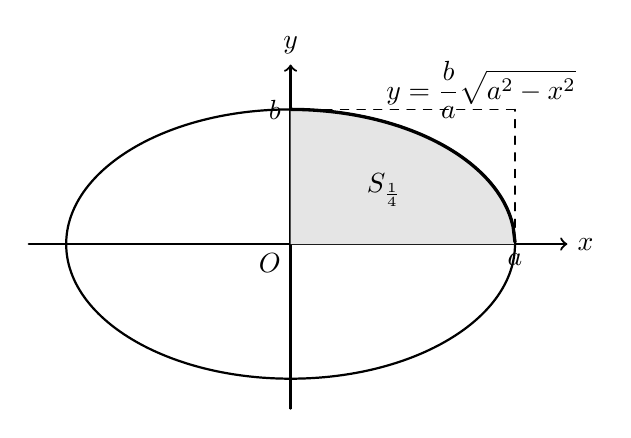
\begin{tikzpicture}[scale=0.95, line cap=round, line join=round]
    % 参数：为了画图美观，这里取 a=3, b=1.8
    \def\a{3}
    \def\b{1.8}

    % 坐标轴
    \draw[->, thick] (-3.5,0) -- (3.7,0) node[right] {$x$};
    \draw[->, thick] (0,-2.2) -- (0,2.4) node[above] {$y$};

    % 椭圆
    \draw[thick] (0,0) ellipse ({\a} and {\b});

    % 第一象限阴影区域
    \fill[gray!20, domain=0:\a, samples=120]
        (0,0)
        --
        plot (\x, {\b*sqrt(1-(\x*\x)/(\a*\a))})
        --
        (\a,0)
        --
        cycle;

    % 第一象限上边界加粗
    \draw[very thick, domain=0:\a, samples=120]
        plot (\x, {\b*sqrt(1-(\x*\x)/(\a*\a))});

    % 辅助线
    \draw[dashed] (0,\b) -- (\a,\b);
    \draw[dashed] (\a,0) -- (\a,\b);

    % 原点与半轴标注
    \node[below left] at (0,0) {$O$};
    \node[below] at (\a,0) {$a$};
    \node[left] at (0,\b) {$b$};

    % 面积标注
    \node at (1.25,0.72) {$S_{\frac14}$};

    % 方程标注
    \node[above right] at (1.15,1.55)
    {$\displaystyle y=\frac{b}{a}\sqrt{a^2-x^2}$};
\end{tikzpicture}

\vspace{0.5em}
\small 图：椭圆第一象限面积的积分表示
\end{center}

设椭圆第一象限部分面积为 $S_{\frac14}$，则
\[
S_{\frac14}
=
\int_0^a y\,dx
=
\int_0^a
\frac{b}{a}\sqrt{a^2-x^2}\,dx.
\]

令
\[
x=a\cos\theta,\qquad 0\le \theta\le \frac{\pi}{2},
\]
则
\[
dx=-a\sin\theta\,d\theta.
\]

当 $x=0$ 时，
\[
a\cos\theta=0,
\]
所以
\[
\theta=\frac{\pi}{2}.
\]

当 $x=a$ 时，
\[
a\cos\theta=a,
\]
所以
\[
\theta=0.
\]

又因为 \(0\le \theta\le \frac{\pi}{2}\)，所以 \(\sin\theta\ge 0\)。于是
\[
\sqrt{a^2-x^2}
=
\sqrt{a^2-a^2\cos^2\theta}
=
\sqrt{a^2\sin^2\theta}
=
a\sin\theta.
\]

于是
\[
\begin{aligned}
S_{\frac14}
&=
\int_0^a
\frac{b}{a}\sqrt{a^2-x^2}\,dx \\[0.5em]
&=
\int_{\frac{\pi}{2}}^0
\frac{b}{a}\cdot a\sin\theta
\cdot
\left(-a\sin\theta\right)
\,d\theta \\[0.5em]
&=
ab\int_0^{\frac{\pi}{2}}\sin^2\theta\,d\theta.
\end{aligned}
\]

由二倍角公式
\[
\sin^2\theta=\frac{1-\cos 2\theta}{2},
\]
可得
\[
\begin{aligned}
S_{\frac14}
&=
ab\int_0^{\frac{\pi}{2}}
\frac{1-\cos 2\theta}{2}
\,d\theta \\[0.5em]
&=
ab
\left[
\frac{\theta}{2}
-
\frac{\sin 2\theta}{4}
\right]_0^{\frac{\pi}{2}} \\[0.5em]
&=
ab
\left(
\frac{\pi}{4}-0
\right) \\[0.5em]
&=
\frac{\pi ab}{4}.
\end{aligned}
\]

因此椭圆总面积为
\[
S
=
4S_{\frac14}
=
4\cdot \frac{\pi ab}{4}
=
\pi ab.
\]

\medskip
\textbf{\textcolor{CProof}{结论回扣}}

\textbf{椭圆 $\frac{x^2}{a^2}+\frac{y^2}{b^2}=1$ 围成区域的面积为 $S=\pi ab$。这里 $a>0,\ b>0$ 是两条半轴长度，公式只看半轴乘积，不要求 $a>b$。}
\end{proofbox}